\section{Methods}
In this part, we will make the notion that $transition = (s, a, s')$, which means that the state $s$ will transition to $s'$ if the action is $a$. 

% ------------------------------------
\subsection{Score Function}
\label{score function}
In our methods mentioned in the introduction, most of them need a score function to evaluate whether the taken action is preferable or not. As a result, how to design a reasonable and effective score function is significant. During all the different methods, the factors that affect the score function are similar. The influencing factors are:
\begin{enumerate}
    \item \textbf{The number of pieces that survived} Since the condition that we don't lose is that we still have pieces that survive on the board, so we should try to make more of our pieces survive. Meanwhile, our movements aim to eat all the pieces of the opponent, so the fewer of the opponent's pieces are, the better the state is. So the number of pieces that survived, both our pieces and the opponent's pieces, matters.
    \item \textbf{The number of kings that exist} Since the king can go backward rather than the non-king piece which can only go forward, the number of kings should be considered in the score function. We should try to make the number of our kings bigger and the number of the opponent's kings smaller.
    \item \textbf{The sum of our all non-king pieces' distances to the opponent's bottom line of the board} Since we need to make more of our kings, the sum of our all non-king pieces' distances to the opponent's bottom line of the board reflects the potential to have more kings. The smaller the sum of distances is, the bigger the potential will be. 
    \item \textbf{The sum of our all pieces' distances to the left or right line of the board} Considering the piece which is next to the left or right line cannot be eaten, we can try to move more pieces to the positions that are next to the left or right line of the board. We can measure this feature by the sum of all pieces' distances to the left or right line of the board, while the distance of pieces next to the left or right line is zero. The smaller the sum of distances is, the better the situation is.
\end{enumerate}
Although different methods differ in the process of getting the best action, as they share the same influencing factors, they can use the same score function to evaluate one state. In most of our methods, the score function we use is:\\
\begin{equation}
\begin{aligned}
f(s) &= \omega_1*(N_{\text{our-survived}}-N_{\text{opponent-survived}})
\\ &+\omega_2*(N_{\text{our-kings}}-N_{\text{opponent-kings}})
\\ &+\omega_3*\sum\limits_{\text{our non-king pieces}}\frac{1}{L_{\text{dis-to-bottom}}}
\\ &+\omega_4*\sum\limits_{\text{our pieces}}\frac{1}{min(L_{\text{dis-to-left}}, L_{\text{dis-to-right}})+1}
\end{aligned}
\end{equation}
where $N$ means the number of pieces, and $L$ means the distance between the selected piece and the target line. What's more, since every non-king piece's distance to the bottom line is not zero, the denominator of the third feature is not zero. But the sum of the minimal distance of each piece to the left or right line may be zero. So we can add 1 to the denominator of the fourth feature to avoid the infinity value of the score function. $\omega_1$ to $\omega_4$ is the weights of each feature. In our implementation, the parameters we use are $\omega_1=1,\omega_2=2,\omega_3=1,\omega_4=0.5$.

% ------------------------------------
\subsection{Random}
A naive but fast agent for a draught game is a random agent, for a given game board and given turns, we could get all possible moves, then we randomly choose one and perform the move. Note that for other games, random agents will perform extremely poorly. But for draught, due to the special rule, that piece must eat the opponent piece if available and small game board, the random agent's performance is not so bad, and it is an ideal agent for fast testing with other types of agents. 

% ------------------------------------
\subsection{Greedy}
A simple improvement of the search agent is a greedy method. For the current state, firstly we get all the valid actions. For each action, we can get the state after movement. Then we can use the score function in section \textbf{Score Function} to get the reward of each state. Then we choose the action with the highest score. Thus, we achieve the best local solution of depth one.

% ------------------------------------
\subsection{Minimax Search}
As a two-player game, a straightforward and efficient method to solve the draught is adversarial search. Here we deploy minimax search to draught, each time the agent finds the optimal search with the assumption that the opponent will move optimally. We implement this algorithm recursively, and to limit the time of each search, we limit the maximum search steps. When the algorithm stops the search, we use the score function to evaluate the current game board score to choose the optimal move. 

We also apply the alpha-beta pruning algorithm to decrease the nodes of the search tree, by pruning nodes with bad performance, we could increase the search depth in a limited time, thus improving the performance. 

% ------------------------------------
\subsection{Reinforcement Learning}
\subsubsection{Monte-Carlo Tree Search}
MCTS (Monte-Carlo Tree Search), a well-known algorithm used in Alpha-GO, could handle large state space problems and complex decision trees. Here we apply MCTS to classical draught games. As shown in figure \ref{fig:mcts}, the MCTS algorithm builds the search tree during the iterations of four steps: Selection, Expansion, Simulation, and Backpropagation. To build the tree, we define our tree structure with tree nodes. For each node, we store the visit time, win time, and parent and children. For the current node, we could use the rule of draught to find all possible movements as the children of the node. Then we explain the details of the four steps. 
\begin{figure}[t]
    \centering
    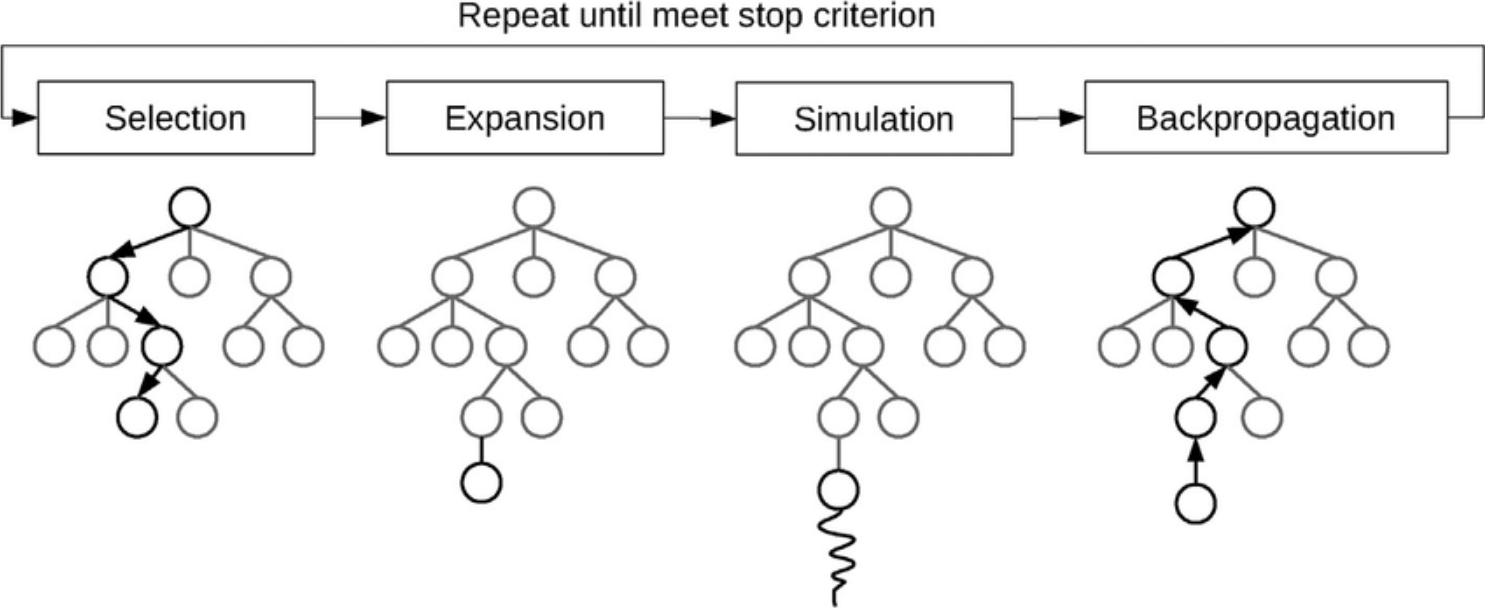
\includegraphics[width=\linewidth]{figures/mcts.png}
    \caption{Illustration of the MCTS algorithm steps}
    \label{fig:mcts}
\end{figure}
\begin{enumerate}
    \item \textbf{Selection} We start from the root node of the search tree, representing the current state of the game, where we use board class to store the current game state. Then we use the UCT (Upper Confidence Bound for Tree) selection policy to select child nodes. The UCT is an application of UCB, and the value can be obtained by $$\mathop{\arg\max}\limits_{v' \in {\rm children \, of} v} \dfrac{Q(v')}{N(v')} + c \sqrt{\dfrac{2 lnN(v)}{N(v')}}$$ where $v$ represents for the parent node, $v'$ is one of the child node of $v$, $N$ is the nodes' visit time, and $Q$ is the quality value of the current node. Note that c is chosen as $\frac{1}{\sqrt{2}}$ as an empirical constant. Each time we select the node with maximum UCT value, by selecting iteratively, we find the leaf node of the search tree that hasn't been fully expanded as a result of the selection step. 
    \item \textbf{Expansion} After selecting a leaf node, we generate child nodes for the current node of possible future states, and then we add these nodes as the child nodes of the leaf node. 
    \item \textbf{Simulation} After Expansion, we perform a simulation of one of the added child nodes. Here we randomly choose actions in the simulation step to estimate the possible final state of the current node. Note that for the speed of the agent, we will limit the max actions step, so if the node needs large steps to get the final state, we will end this step ahead and regard the player that has more pieces as the winner. 
    \item \textbf{Backpropagation} Lastly, we perform backpropagation through the tree to update all parent nodes of the search path. We update the visit times and the reward of win or lose to each node.
\end{enumerate}
As for an MCTS agent, we first initialize a state class to store the current state of the game, then we perform the four steps for fixed iterations. After building the tree for search, we choose the best child of the current node by finding the maximum layouts and return the corresponding best action. With a larger number of iterations, the tree is built more richly, thus the agent will be more intelligent. However increasing the number of iterations will also result in longer inference time, so a balance between iterations and intelligence is important. 

% ------------------------------------
\subsubsection{Q-Learning}

Q-learning is a reinforcement learning approach, we hope we can learn a better strategy while taking action. 
We define the Q value($Q(s, a)$) as the current state which is represented by the current board, and the action which is represented by the next board because we are dealing with a determinate action. Besides, we use the evaluate function mentioned in section \textbf{Score Function} to define the reward in two different ways.

$$r1(s,a,W) = f(s,W) - f(s',W) $$
$$r2(s,a,W) = [f(s,W) - f(s',W)] - [f(s',B) - f(s'',B)]$$

where $f$ is the evaluate function, $s$ is the current board, $s'$ is the next board, $s''$ is the board after the opponent's action, and we are WHITE as an example. Specifically, we get a positive reward if we eat pieces, move toward the opponent, or win. The two ways differ mainly in whether we consider the opponents' reward. Experiments show that they are almost the same and the second one is a bit better.
% More comparison experiments will be shown in Section $\textbf{Result}$.

Considering the training, we train our agents against random agents. As we take an action, we have a new sample and we use the sample to update our Q-value, the procedure is as follows:

$$sample = r1(s,a,W) + \gamma \mathop{\max}_{{a'}}  Q(s',a')$$
$$Q(s,a) \gets (1 - \alpha)Q(s,a) + \alpha (sample)$$

As to the parameters, we also have ideas and experiments. $\gamma$ is the discounting factor that decides whether we prefer early reward. In Draught, there is a special rule which is ``must eat when you can eat", so a strategy that we can sacrifice a piece to control the opponent's action, thus benefiting long-term situation may exist, which makes the discounting factor $\gamma>1$ possible. Based on this we try the discounting factor from $0.8$ to $1.1$. The results show that $0.8$ works better and we think the main reason lies in that the agent's intelligence now didn't reach the level that may consider such a complex strategy. Moreover, we set $\epsilon$ to $0.4$ to enable our agent to explore more states. However, when testing, we still have problems that we possibly meet an unvisited Q-state and we can only regard its Q-value as $0$.

\subsubsection{Approximate Q-Learning}

Since there are a total of $5^{32}\approx10^{22}$ states, it is not possible to visit all as long as store all states during training. So we introduce the approximate Q-learning to avoid the side effects of unvisited states.

Our experience is summed up in a few powerful numbers. We take the following experimental value functions for approximate Q-values.

\begin{equation}
f_1(s, a) = \left\{\begin{aligned}
10 &, \text{if the WHITE side wins}\\
-10 &, \text{if the BLACK side wins}\\
0&,  \text{otherwise}\\
\end{aligned}\right. \\
\end{equation}
$$f_2(s,a)=N_{\text{our-survived}}  +\ 2*N_{\text{our-kings}}$$
all $N$ are numbers for state $s$

\begin{equation}
    f_3(s, a) = \sum\limits_{\text{our non-king pieces}\in s}\frac{1}{L_{\text{dis-to-bottom}}}
\label{f3}
\end{equation}
all $L$ are depth for state $s$

$$
f_4(s,a) = \sum\limits_{\text{our pieces}\in s}\frac{1}{min(L_{\text{dis-to-left}}, L_{\text{dis-to-right}})+1}
$$

Where $N$ means the number of pieces, and $L$ means the distance between the selected piece and the target line. All former formulas are only considered the state $s$.

We also need to take the state after the transition into consideration, by setting
$$f_5(s,a) = -f_1(s,a)$$
$$f_6(s,a)=N_{\text{opponent-survived}} + 2 * N_{\text{opponent-kings}}$$
all $N$ are numbers for state $s'$

\begin{equation}
    f_7(s, a) = \sum\limits_{\text{our non-king pieces}\in s'}\frac{1}{L_{\text{dis-to-bottom}}}
\end{equation}
all $L$ are depth for state $s'$

$$
f_8(s,a) = \sum\limits_{\text{our pieces}\in s'}\frac{1}{min(L_{\text{dis-to-left}}, L_{\text{dis-to-right}})+1}
$$

With the constructed value functions for approximate Q-values above, we could train with the method of approximate Q-learning:

$$sample = \sum_{i=1}^8w_if_i(s,a)$$
$$difference = sample - Q(s,a)$$
$$Q(s,a) \gets (1 - \alpha)Q(s,a) + \alpha (sample)$$
$$w_i \gets w_i + \alpha (difference)f_i(s,a)$$

For the training details, we set the discount factor $\gamma=0.8$, and all weights $w_i$ are initially set to be $10$. We firstly pre-train the model, we totally trained $3000$ epochs, with a learning rate to be $0.01$, and after the $1000$-th epoch, the learning rate times $0.99$ after each epoch. The opponent to be the minimax search with depth $3$.

Then we do finetune for the pre-trained model, similar to the pre-training, but we set the learning rate to be $0.001$ at initial, and the opponent to be the minimax search with depth $5$.

After finetuning, we tested the winning rate for our trained approximate Q-learning model, the winning rate has a great increase compared to the pretraining model. The winning rate of Approximate Q-learning and random increases from $89\%$ increase to $91\%$.

% ------------------------------------
\subsubsection{Neural Network}

Since testing the Minimax algorithm could generate a large amount of battle information, we want to make good use of it. By using the previous battle information to train a Neural Network, and generate a new feature for the \textbf{Approximate Q-learning}.

We collected the training data by storing the match information during testing the winning rate between Minimax with depth $7$ and another Minimax with depth $7$.
We store each board's information and the turn of the player during the matching. After matching, the board that was generated by the winner is set to have the label $+1$, and the board that was generated by the loser is set to have the label $-1$. Also, the board's generator was also recorded.

With the generated data, we could do training and inference to generate the new feature for approximate Q-learning.

\begin{figure}[t]
    \centering
    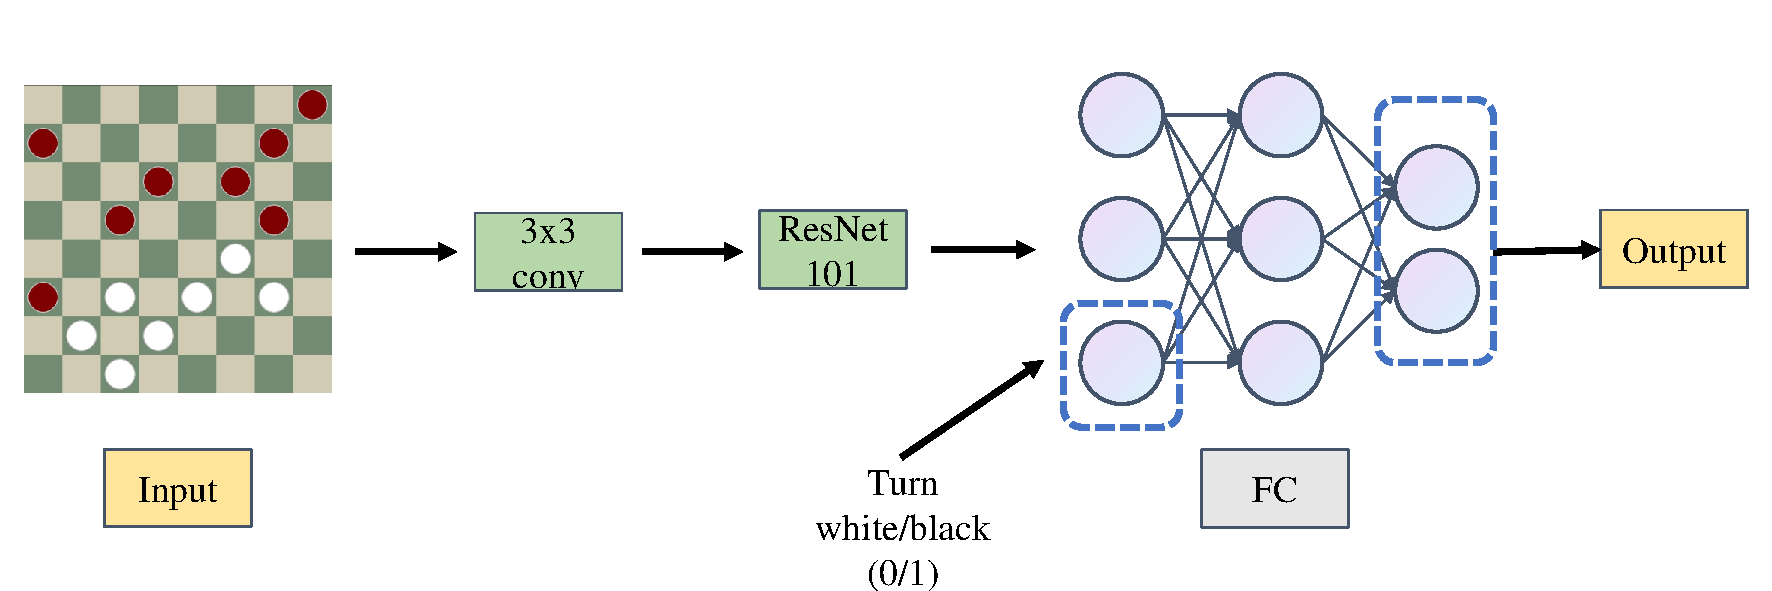
\includegraphics[width=\linewidth]{figures/neural.pdf}
    \caption{The pipeline of the Neural Network to generate new features.}
    \label{fig:pipeline}
\end{figure}

\begin{enumerate}
    \item \textbf{Training}
    Throw our observation during the matchings, almost all capture operations happened within $2$ steps. This means that in nearly all situations if a piece eats the opponent's pieces, it will not eat more than $2$ pieces. So if we consider the board as an image, a convolution kernel with $5\times 5$ receptive field is enough.

    After the convolution layer, we set ResNet101 and a $3$-layer fully connected MLP to do the $ 2$ classification task. The output layer includes two numbers since we are doing the $ 2$ classification, so the final output $+1$ or $-1$ is the prediction of the new state's winning rate. And we set this to be the new feature for approximate Q-learning.
    
    The total pipeline is shown in \ref{fig:pipeline}.
    
    \item \textbf{Inference} To generate the new feature, we put the origin board $s$, and the board $s'$ after action $a$ respectively into the network, and infer the winning rate. The winning rates are set to be the new feature $f_{new}(s,a)$.

\end{enumerate}

After generating the new feature, we put it into the original \textbf{Approximate Q-learning}, all settings are the same instead of adding a feature. And we could see that the winning rate has increased. The details are shown in Section \textbf{Result}.